 A function is said to be convex if following inequality is true:
\begin{align}
    \lambda f(x_1)+(1-\lambda) f(x_2) \geq f(\lambda x_1+(1-\lambda) x_2)
\end{align}
and for $\lambda \in [0,1]$
\begin{align}
&\lambda(9x_1^2+12x_1+2)+(1-\lambda)((9x_2^2+12x_2+2) \geq \nonumber \\ 
&9(\lambda x_1 +(1-\lambda )x_2)^2+12(\lambda x_1 +(1-\lambda )x_2)+2\\
&x_1^2(9\lambda-9\lambda^2)+x_2^2(9\lambda-9\lambda^2)-2x_1x_2(9\lambda-9\lambda^2) \geq 0\\
&(9\lambda-9\lambda^2)(x_1^2+x_2^2-2x_1x_2)\\
&9\lambda(1-\lambda)(x_1-x_2)^2 \geq 0 \label{eq:solutions/5/2/1/2/eq:2}
\end{align}
Equation \eqref{eq:solutions/5/2/1/2/eq:2} holds true for all $\lambda\in(0,1)$. Hence the given function f(x) is convex.
 Fora general quadratic equation
\begin{align}
    f(x)=ax^2+bx+c
\end{align}
The update equation for gradient descent to find minimum of a function is given by:
\begin{align}
    \lambda_{n+1}=\lambda_n-\mu f'(\lambda_n) 
%\label{eq:solutions/5/2/1/2/eq:2}
\\
    =\lambda_n-\mu (2a\lambda_n +b)
\end{align}
In equation \eqref{eq:solutions/5/2/1/2/eq:2} $\lambda_0$ is an initial guess and $\mu$ is a variable parameter,known as step size $\lambda_{n+1}$ is the next position. The minus sign refers to the minimization part of gradient descent.
 Assume,
\begin{align}
    \lambda_0=1\\
    \mu=0.001 \\
    precision = 0.00000001\\
    \implies \lambda_1=1-0.001(2\times9\times1+12)\\
    \implies \lambda_1=1-0.03\\
    =0.97
\end{align}
following the above method, we keep doing iterations until $\lambda_{n+1}-\lambda_{n}$ becomes less than the value of precision we have chosen.
{Results}
Using python, the results are:
\begin{enumerate}
	\item The local minimum occurs at -0.666666130125316.
	\item The value of f(x) at minima is -1.9999999999974087
\end{enumerate}
Figure \ref{eq:solutions/5/2/1/2/Fig:1} shows plot of parabola obtained from python code:
\begin{figure}[h]
\renewcommand{\theenumi}{1}
\centering
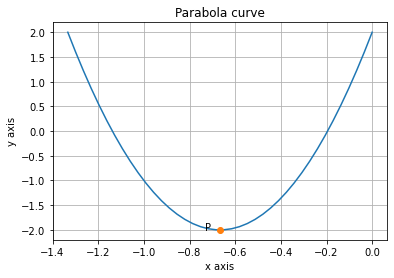
\includegraphics[width=\columnwidth]{./solutions/5/2/1/2/Parabola.png}
\caption{Plot obtained from python code}
\label{eq:solutions/5/2/1/2/Fig:1}
\end{figure}
